\documentclass{article}

% --- 1. Encoding & Fonts ---
\usepackage[T1]{fontenc}
\usepackage{microtype}      % Improves spacing/kerning

% --- 2. Math & Symbols ---
\usepackage{amsmath, amssymb, amsthm, amsfonts} % Core math
\usepackage{mathtools, bm, bbm}                 % Tools, bold math, indicator 1
\usepackage{textcomp} % Fix warning
\usepackage{nicefrac, gensymb, chngcntr}        % Fractions, degree symbol, counters

% --- 3. Figures & Graphics ---
\usepackage{graphicx, wrapfig, placeins}        % Images, wrapping, FloatBarrier
\usepackage{caption, subcaption}                % Caption formatting
\usepackage{tikz, color}                        % Drawing & Color (epsfig removed)
\graphicspath{{../outputs/}}

% --- 4. Tables & Lists ---
\usepackage{booktabs, multirow, makecell}       % Prof. tables, spanning rows/cells
\usepackage{enumitem}                           % Customizable lists
\usepackage{url}                                % URL formatting

% --- 5. Hyperref (Must load BEFORE ICML style) ---
\usepackage{hyperref}

% --- 6. ICML Style (Loads natbib automatically) ---
% Replace 'icml2024' with your specific year (e.g., icml2025, icml2026)
% usepackage[accepted]{icml2024} % Use [accepted] if camera-ready
\usepackage[accepted]{icml2026}


\newcommand{\commento}[1]{\textcolor{red}{[\textit{#1}]}} \newcommand{\ting}[1]{\textcolor{red}{[TC: \textit{#1}]}} \newcommand{\mohammad}[1]{\textcolor{blue}{(MN: #1)}}
\newcommand{\todo}[1]{\textcolor{red}{[\textit{TODO: #1}]}} 

\DeclareMathOperator*{\argmax}{arg\,max}
\DeclareMathOperator*{\argmin}{arg\,min}

\newtheorem{theorem}{Theorem}
\newtheorem{definition}{Definition}
\newtheorem{lemma}[theorem]{Lemma}
\newtheorem{corollary}{Corollary}\newtheorem{proposition}{Proposition}\newcommand{\one}[1]{\mathbbm{1}_{[#1]}}

\makeatletter
\renewcommand{\ICML@appearing}{}
\makeatother


\begin{document}

\twocolumn[
  \icmltitle{Bridging the Semantic Gap in Healthcare: \\ A Comparative Analysis of RAG and HyDE}

  \icmlsetsymbol{equal}{*}

  \begin{icmlauthorlist}
    \icmlauthor{Sergio Herreros Pérez}{icai}
    \icmlauthor{Adrián López-Lanchares Echezarreta}{icai}
    \icmlauthor{Ignacio Bayón Jiménez-Ugarte}{icai}
  \end{icmlauthorlist}

  % corresponding author
  \icmlcorrespondingauthor{Sergio Herreros Pérez}{sergio.herreros@alu.comillas.edu}
  \icmlcorrespondingauthor{Adrián López-Lanchares Echezarreta}{adrianlanchares@alu.icai.comillas.edu}
  \icmlcorrespondingauthor{Ignacio Bayón Jiménez-Ugarte}{ibayon@alu.comillas.edu}

  \icmlaffiliation{icai}{Master in Artificial Intelligence, Universidad Pontificia Comillas (ICAI)}

  \icmlkeywords{World Models, Imagination, Reinforcement Learning}

  \vskip 0.3in
]
\setlength{\textfloatsep}{0.15in}

\printAffiliationsAndNotice{}

\begin{abstract}
  Large Language Models (LLMs) using Retrieval-Augmented Generation (RAG) struggle with the vocabulary mismatch between everyday medical queries and complex clinical texts. This paper evaluates Hypothetical Document Embeddings (HyDE) to bridge this semantic gap within a Qwen2.5 7B ReAct agent. Using a custom Medline-based dataset, we demonstrate that while HyDE significantly improves retrieval accuracy for medical jargon and rare diseases, it introduces a substantial 41\% latency overhead. Conversely, standard RAG achieves parity on symptom descriptions and common terms. We conclude that medical agents must employ dynamic query routing to balance HyDE's precision with RAG's efficiency.\footnote{Code and data are available at: \url{https://github.com/adrianlanchares/reasoning-tool-llm-agent}}
\end{abstract}

\section{Introduction}
\label{sec:introduction}

Large Language Models (LLMs) demonstrate remarkable reasoning capabilities but risk hallucination in specialized domains like healthcare. Retrieval-Augmented Generation (RAG) mitigates this by grounding responses in external databases, conceptually separating internal memory from factual retrieval.

However, standard RAG architectures suffer from a critical vocabulary mismatch when applied to highly specialized medical databases. A severe gap in meaning often exists between everyday user queries (e.g., "stomach bug") and formal clinical documentation (e.g., "gastroenteritis"). Consequently, standard search models frequently fail to bridge this gap, resulting in poor retrieval and depriving the reasoning agent of the necessary context to form a safe, accurate diagnosis.

To address this limitation, recent advancements have proposed Hypothetical Document Embeddings (HyDE) \citep{gao2022hyde}. HyDE bypasses the vocabulary gap by changing the search approach to document-to-document matching. By prompting the base LLM to generate a hypothetical, medically-styled document in response to the user's query, the system captures the expected clinical vocabulary and linguistic patterns prior to executing the database search. 

In this paper, we systematically evaluate the efficacy of HyDE against a standard RAG baseline within an autonomous ReAct (Reason + Act) agent architecture \cite{yao2023react}. Powered by Qwen2.5 7B and grounded in a highly preprocessed subset of the Medline dataset \cite{medlineplus}, we stress-test this vocabulary gap using a custom synthetic dataset curated across four categories: Common Terms, Symptoms, Medical Jargon, and Rare Diseases.

Our comprehensive evaluation demonstrates that while HyDE significantly improves retrieval accuracy for complex jargon and rare diseases, it introduces a substantial computational overhead, increasing processing latency. Furthermore, we reveal that HyDE is not universally required; the robust internal knowledge of the Qwen2.5 base model allows standard RAG to achieve performance parity on dense symptom descriptions and everyday terms. These findings underscore the necessity of dynamic query routing in production-grade medical agents, balancing the precision of HyDE against the computational efficiency of standard RAG.

\section{Background}\label{sec:background}

\subsection{Before RAG: The Limits of Standalone Language Models}
Historically, applying large language models to specialized tasks relied heavily on the knowledge stored directly within the model's own weights during training. While this approach—often enhanced through supervised fine-tuning or reinforcement learning—allows models to reason and format answers well, it presents significant drawbacks for knowledge-intensive fields like medicine. A standalone model cannot easily update its knowledge without expensive retraining. More importantly, when asked about highly specific or rare medical conditions, models relying solely on internal memory are prone to hallucination, generating answers that sound confident but lack factual accuracy.

\subsection{RAG and the Challenge of Domain-Specific Search}
To address the limitations of standalone models, Retrieval-Augmented Generation (RAG)~\cite{lewis2021rag} was developed. RAG improves a model's accuracy by searching an external database for relevant facts and providing that text to the model before it answers. While fundamental RAG pipelines effectively retrieve general knowledge, applying them to highly specialized, massive databases presents unique challenges. Standard RAG relies on matching a user's raw question to target documents in a shared space. However, in medical contexts, user queries are often brief or phrased differently than formal clinical texts, creating a gap in meaning. As a result, standard search models frequently struggle to connect simple queries to documents containing rare medical terminology. This vocabulary mismatch leads to poor search results, leaving the reasoning agent without the necessary context to form an accurate answer.

\subsection{Hypothetical Document Embeddings (HyDE)}
To overcome the vocabulary limitations of standard RAG, advanced systems implement Hypothetical Document Embeddings (HyDE) as a search extension~\cite{gao2022hyde}. HyDE bypasses the gap between the user's simple query and the complex source document by shifting the approach to document-to-document matching. Instead of directly searching with the user's initial prompt, the system uses a language model to generate a hypothetical document in response to the question. While this generated text might contain factual inaccuracies, it successfully captures the expected language patterns, clinical vocabulary, and keywords naturally associated with the medical topic. Searching the database with this medically styled document significantly improves the retrieval of relevant information compared to using the raw question.

\subsection{The Medline Dataset}
In this project, the external knowledge base is grounded in Medline, a premier bibliographic database containing millions of references to journal articles in the life sciences and biomedical fields\cite{medlineplus}. Medline serves as an authoritative source of medical knowledge, covering everything from common treatments to rare diseases and complex pharmacology. However, the language used in Medline articles is highly technical, dense, and formal. This makes it an ideal testing ground for advanced retrieval techniques like HyDE, as successfully navigating Medline requires bridging the gap between everyday user questions and deeply specialized medical literature.

\section{Methodology}
\label{sec:methodology}

To quantitatively evaluate the effectiveness of HyDE in mitigating the vocabulary mismatch problem inherent to standard RAG, we designed an end-to-end evaluation pipeline. This pipeline leverages a custom-curated synthetic dataset mapped to MedlinePlus Health Topics and computes both retrieval accuracy and computational overhead metrics. To empirically test the theoretical vocabulary gaps identified in the Medline corpus, we designed an end-to-end evaluation pipeline.

\subsection{Synthetic Dataset Curation}
While large-scale consumer health datasets such as MedQuAD \citep{benabacha2019medquad} provide extensive mappings of medical queries to MedlinePlus documents, their queries are largely template-driven (e.g., ``What is [Disease]?''). These highly lexical queries fail to expose the primary vulnerability of standard semantic search: the semantic gap between patient colloquialisms and clinical documentation. To explicitly stress-test this gap, we curated a custom evaluation dataset of 25 targeted queries. Each query is manually mapped to an exact, verifiable MedlinePlus Health Topic.

The dataset is intentionally stratified into four distinct categories to isolate and measure specific retrieval vulnerabilities:

\noindent\textbf{Colloquialisms / Layman Terms.} This category tests the model's ability to map common, non-medical phrases to their clinical counterparts. For example, it evaluates whether the system can map ``stomach flu'' to the target topic \textit{Gastroenteritis}, bypassing the literal text embedding of the word ``flu.''

\noindent\textbf{Symptom-to-Diagnosis.} Queries in this category are highly contextual, multi-sentence narratives describing a cluster of symptoms (e.g., painful urination and pelvic heaviness). This evaluates whether HyDE can synthesize a hypothetical diagnosis (e.g., \textit{Urinary Tract Infections}) prior to retrieval, whereas standard RAG typically retrieves generic pages clustered around surface-level terms like ``pain.''

\noindent\textbf{Medical Jargon.} This category serves as a reverse-dictionary test. Because MedlinePlus utilizes consumer-friendly titles, queries leveraging strict clinical terminology (e.g., ``epistaxis'') must be conceptually bridged to their layman equivalents in the database (e.g., \textit{Nosebleed}).

\noindent\textbf{Rare Diseases.} This category serves as a stress test for the base Large Language Model's (LLM) internal parametric knowledge. It evaluates the model's capacity to generate accurate hypothetical documents for niche genetic conditions or rare disorders based purely on complex symptomatic descriptions.

\subsection{Data Ingestion and XML Preprocessing}

To effectively populate the Chroma vector database, the raw Medline dataset required targeted preprocessing. The original XML corpus contained substantial metadata and relational tags (e.g., \texttt{<related\_pages>}) that act as navigational noise, which can degrade the semantic quality of dense embeddings.

Using a custom parsing pipeline (via \texttt{ingest\_data.py}), we isolated only the high-signal clinical text. By extracting core medical content---such as titles, body text, and summaries---and systematically stripping away structural tags, internal IDs, and formatting metadata, we ensured the sentence-transformer model processed purely factual knowledge. This cleaning process optimized the resulting vector space, enabling the ReAct agent's retrieval tool to match hypothetical documents against clean clinical data.

\subsection{Experimental Pipeline}
We deployed two parallel API endpoints: a Classic RAG pipeline and a HyDE-augmented pipeline. To ensure deterministic generation of the hypothetical documents and to prevent hallucinatory variance across evaluation runs, the base LLM temperature for the HyDE generation step was strictly set to $T=0$ (greedy decoding).

For each query in the dataset, the prompt is dispatched to both endpoints. The evaluation script captures the full execution trace of the LLM agent, isolating the intermediate tool call outputs (e.g., \texttt{rag\_retrieve\_context}).

\textbf{Transition to Exact URL Validation.}
Initially, retrieval success was calculated using a case-insensitive substring match between the predefined target topic and the titles of the top $k=3$ retrieved documents. However, manual auditing of the ReAct trace revealed that this approach introduced significant false positives due to spelling similarities, particularly across languages. For example, when evaluating Query 23 regarding the eating disorder \textit{Pica}, the standard RAG pipeline mistakenly retrieved Spanish-language documents concerning ``Picaz\'{o}n'' (Itching) and ``Picaduras de ara\~{n}as'' (Spider bites). Because the string ``pica'' is a literal substring of these terms, the naive evaluator incorrectly recorded a perfect retrieval hit.

To eliminate these false positives and ensure rigorous evaluation, we abandoned substring matching. Our finalized pipeline relies exclusively on exact URL validation. A successful retrieval is now only recorded if the unique MedlinePlus URL associated with the target topic is strictly matched within the context chunks returned by the vector database.

\subsection{Evaluation Metrics}
To provide a holistic comparison between standard RAG and HyDE, we evaluate the models across four dimensions, balancing retrieval accuracy against computational cost.

\noindent\textbf{Hit Rate @ $k$.} We define Hit Rate @ 3 as a binary metric indicating whether the exact target MedlinePlus topic appears within the top $k=3$ retrieved documents. This metric reflects the absolute success rate of the retrieval step.

\noindent\textbf{Mean Reciprocal Rank (MRR).} To account for the positional relevance of the retrieved documents, we compute the MRR. The rank $r_i$ represents the position (1, 2, or 3) of the target topic in the retrieved list for query $i$. If the topic is not retrieved, the reciprocal rank is 0. This metric heavily penalizes systems that retrieve the correct document but bury it at the bottom of the context window. It is computed as:
$$ \text{MRR} = \frac{1}{|Q|} \sum_{i=1}^{|Q|} \frac{1}{r_i} $$
where $|Q|$ is the total number of queries in the dataset.

\noindent\textbf{End-to-End Latency.} We measure the total generation time (in seconds) from the initial dispatch of the HTTP request to the receipt of the final JSON response. This metric captures the temporal overhead introduced by HyDE's requisite intermediate generation step.

\noindent\textbf{Token Usage.} To quantify the computational and financial cost, we record the total tokens consumed per query. For the HyDE pipeline, this explicitly includes the token cost of the ``think'' phase—the generation of the hypothetical document—prior to the vector database search.
\section{Results}
\label{sec:results}

% 1. FULL-WIDTH TABLE
\begin{table*}[t]
    \centering
    \caption{Aggregate Metrics by Category comparing standard RAG and HyDE pipelines.}
    \label{tab:rag_hyde_metrics}
    \begin{tabular}{l r r r r r r r r}
        \toprule
                          & \multicolumn{2}{c}{\textbf{Hit Rate}} & \multicolumn{2}{c}{\textbf{MRR}} & \multicolumn{2}{c}{\textbf{Time (s)}} & \multicolumn{2}{c}{\textbf{Tokens}}                                                                       \\
        \cmidrule(lr){2-3} \cmidrule(lr){4-5} \cmidrule(lr){6-7} \cmidrule(lr){8-9}
        \textbf{Category} & \textbf{RAG}                          & \textbf{HyDE}                    & \textbf{RAG}                          & \textbf{HyDE}                       & \textbf{RAG}   & \textbf{HyDE}  & \textbf{RAG}    & \textbf{HyDE}   \\
        \midrule
        Colloquialism     & 0.83                                  & 0.83                             & 0.75                                  & 0.83                                & 23.70          & 27.48          & 1183.8          & 1310.8          \\
        Medical Jargon    & 0.57                                  & 0.71                             & 0.50                                  & 0.71                                & 18.80          & 20.04          & 1061.3          & 1417.0          \\
        Rare Disease      & 0.33                                  & 0.50                             & 0.33                                  & 0.50                                & 15.98          & 24.73          & 1161.5          & 1721.0          \\
        Symptoms          & 1.00                                  & 1.00                             & 0.81                                  & 0.81                                & 12.76          & 29.74          & 1337.3          & 1876.3          \\
        \midrule
        \textbf{OVERALL}  & \textbf{0.68}                         & \textbf{0.76}                    & \textbf{0.59}                         & \textbf{0.71}                       & \textbf{17.85} & \textbf{25.28} & \textbf{1181.0} & \textbf{1574.7} \\
        \bottomrule
    \end{tabular}
\end{table*}

\subsection{Overall Retrieval Performance}
While the overall absolute performance on our complex synthetic dataset was highly challenging, the implementation of HyDE maintained a clear advantage over the standard RAG baseline. As shown in Table \ref{tab:rag_hyde_metrics}, the overall Hit Rate improved from 0.68 to 0.76, while the Mean Reciprocal Rank (MRR) saw a corresponding increase from 0.59 to 0.71. However, categorizing the queries reveals that HyDE's benefits are heavily dependent on the lexical structure of the user's prompt.

\begin{figure}[ht]
    \centering
    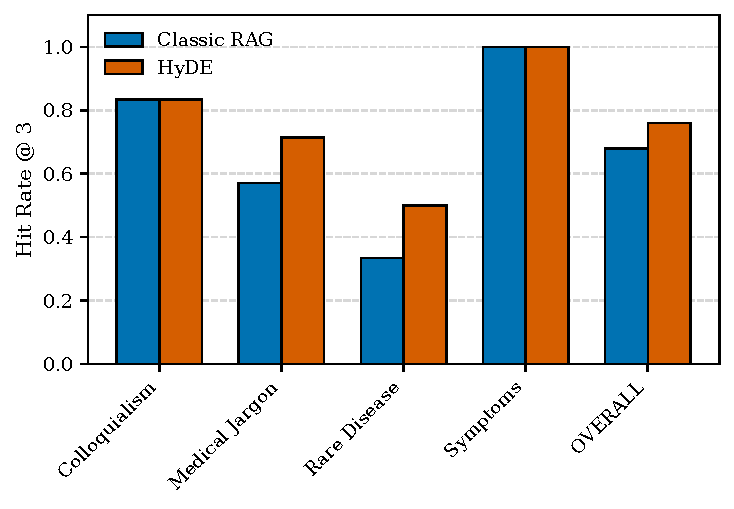
\includegraphics[width=\linewidth]{1_hit_rate_comparison.pdf}
    \caption{Comparison of Hit Rate between standard RAG and HyDE across query categories.}
    \label{fig:hit_rate}
\end{figure}

\subsection{Areas of Parity: Symptoms and Colloquialisms}
Interestingly, standard RAG and HyDE performed identically in two specific categories: Symptoms and Colloquialisms.

For \textbf{Symptoms}, both pipelines achieved a perfect Hit Rate of 1.00 and an MRR of 0.81. This parity is primarily due to the lexical density of symptom-based queries. Because these queries are typically multi-sentence descriptions containing numerous explicit medical keywords (e.g., "pain," "fever," "swelling"), they provide a massive surface area for standard vector search to successfully match against target documents, rendering HyDE's intermediate hallucination step unnecessary.

Similarly, both pipelines achieved a 0.83 Hit Rate for \textbf{Colloquialisms}. This highlights the robust parametric knowledge embedded in our base model (Qwen2.5 7B). The model natively understands common, non-medical terms well enough to bridge the semantic gap to clinical literature without needing a generated hypothetical document to act as an intermediary.

\subsection{HyDE's Edge: Medical Jargon and Rare Diseases}
HyDE proved its worth precisely where the base model and standard retrieval struggled most. In the \textbf{Medical Jargon} category, where queries utilize strict clinical terminology that differs from the consumer-friendly titles in MedlinePlus, HyDE improved the Hit Rate from 0.57 to 0.71, and boosted the MRR from 0.50 to 0.71.

Similarly, for \textbf{Rare Diseases}, standard RAG struggled significantly (0.33 Hit Rate), likely because sparse queries about niche disorders lack the semantic overlap needed to find corresponding documents. By generating a hypothetical document first, HyDE was able to expand the context and improve the Hit Rate to 0.50 (see Figure \ref{fig:mrr}).

\begin{figure}[ht]
    \centering
    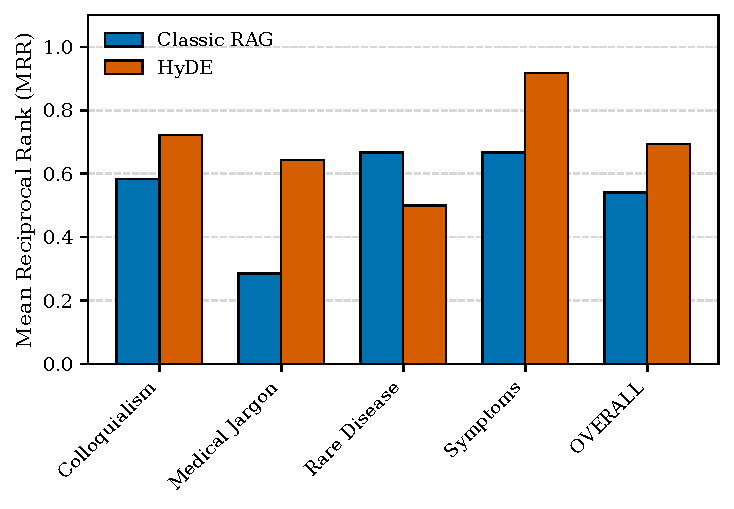
\includegraphics[width=\linewidth]{2_mrr_comparison.pdf}
    \caption{Comparison of Mean Reciprocal Rank (MRR) between standard RAG and HyDE.}
    \label{fig:mrr}
\end{figure}

\subsection{Computational and Latency Trade-offs}
The retrieval improvements observed in the Medical Jargon and Rare Disease categories come at a notable computational cost. Overall mean processing time increased by roughly 41\%, rising from 17.85 seconds with standard RAG to 25.28 seconds with HyDE. This latency is a direct consequence of the sequential "think" phase required to generate the hypothetical document. Token consumption mirrored this trend, increasing from an overall mean of 1181 tokens to 1575 tokens per query. For a detailed visual breakdown of these computational trade-offs across all query categories, please refer to Figure \ref{fig:time_metrics} and Figure \ref{fig:token_metrics} in Appendix \ref{appendix:extra_plots}.

\section{Conclusion and Future Work}
\label{sec:conclusion}

This study evaluated the efficacy of HyDE against a standard RAG baseline within a highly specialized medical domain. Our findings demonstrate that while standard semantic search struggles with the vocabulary mismatch inherent in complex medical jargon and rare diseases, HyDE effectively bridges this gap. By generating an intermediate clinical document, HyDE significantly improved both the Hit Rate and Mean Reciprocal Rank (MRR) for these challenging query categories, equipping the ReAct agent with highly accurate context.

However, our results also highlight that HyDE is not universally necessary. For lexically dense queries---such as multi-sentence symptom descriptions---and common colloquialisms, standard RAG performed equally well as HyDE. This underscores the robust internal knowledge of the base Qwen2.5 7B model, which successfully mapped common terminology to clinical targets without the need for an intermediate generation step. Given the nearly 1.5x increase in generation time and higher token consumption introduced by HyDE, our evaluation suggests that an optimal production system should employ dynamic query routing. Such a system would utilize standard RAG for lexically rich or common queries, reserving the computationally expensive HyDE pipeline exclusively for sparse, jargon-heavy prompts.

While the absolute performance gains of HyDE may appear incremental in certain categories, in the high-stakes domain of healthcare, marginal improvements in retrieval accuracy are critically important. The computational trade-offs are heavily outweighed by the necessity of providing the reasoning agent with the most comprehensive and factually accurate context possible to prevent diagnostic hallucination. We do, however, acknowledge the limitations of evaluating this architecture purely through automated URL matching on a synthetic dataset. To truly gauge clinical viability and safety, the system must undergo rigorous qualitative stress-testing and human-in-the-loop evaluation by licensed medical professionals.

Looking forward, the structural richness of the Medline dataset offers a promising avenue for advancing this retrieval architecture. During our data ingestion phase, we systematically stripped relational XML tags, such as \texttt{<related\_pages>}, to optimize the raw text for dense vector embeddings. However, these discarded tags represent an explicit, human-curated web of medical relationships. Future work will focus on transitioning from standard vector search to a Graph RAG architecture. By embedding the medical documents as nodes and utilizing the \texttt{<related\_pages>} tags as relational edges, an autonomous agent could dynamically traverse this knowledge graph. This would enable multi-hop reasoning, allowing the agent to gather comprehensive, interconnected context for complex diagnostic queries that standard vector similarity currently fails to capture.

% -------------------------
% References
% -------------------------
\bibliographystyle{icml2026}
\bibliography{references}

% -------------------------
% Appendix
% -------------------------
\newpage
\appendix

\section{Additional Computational Metrics}
\label{appendix:extra_plots}

This section provides a detailed visual breakdown of the computational trade-offs introduced by the HyDE extension, specifically regarding processing latency and token consumption.

\begin{figure}[!h]
    \centering
    % Replace 'time_plot.png' with your actual image file name
    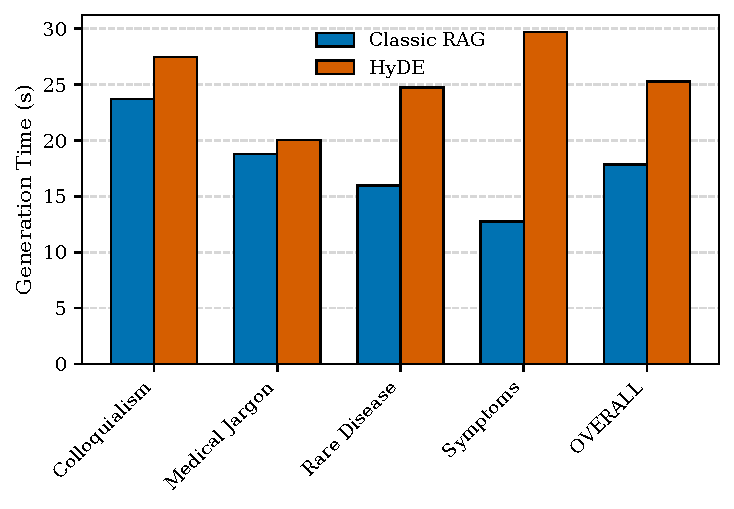
\includegraphics[width=\linewidth]{3_time_comparison.pdf}
    \caption{Comparison of mean processing time (in seconds) between standard RAG and HyDE across different query categories.}
    \label{fig:time_metrics}
\end{figure}

\begin{figure}[!h]
    \centering
    % Replace 'tokens_plot.png' with your actual image file name
    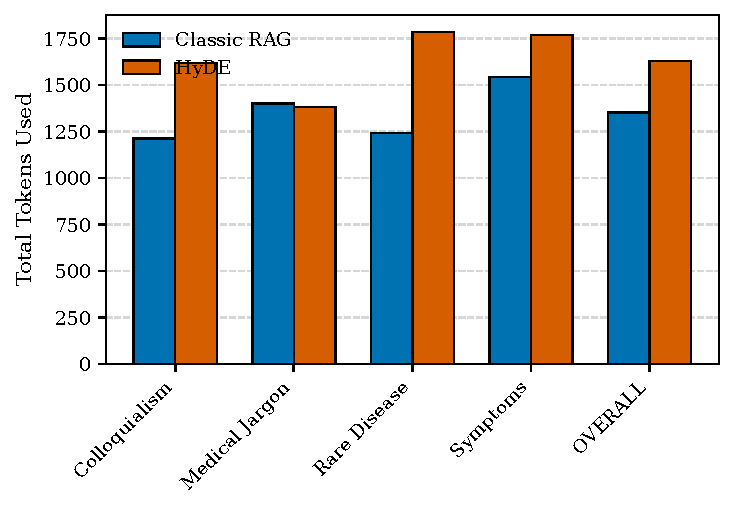
\includegraphics[width=\linewidth]{4_token_comparison.pdf}
    \caption{Comparison of mean token consumption between standard RAG and HyDE across different query categories.}
    \label{fig:token_metrics}
\end{figure}

\end{document}